\let\negmedspace\undefined
\let\negthickspace\undefined
\documentclass{article}
\usepackage{cite}
\usepackage{amsmath,amssymb,amsfonts,amsthm}
\usepackage{algorithmic}
\usepackage{graphicx}
\usepackage{textcomp}
\usepackage{xcolor}
\usepackage{txfonts}
\usepackage{listings}
\usepackage{alphalph}
\usepackage{enumitem}
\usepackage{tfrupee}
\usepackage{mathtools}
\usepackage{gensymb}                                                                                                                                                             \usepackage[breaklinks=true]{hyperref}
\usepackage{tkz-euclide} % loads  TikZ and tkz-base
\usepackage{listings}
\usepackage{gvv}
%
%\usepackage{setspace}
%\usepackage{gensymb}
%\doublespacing
%\singlespacing

%\usepackage{graphicx}
%\usepackage{amssymb}
%\usepackage{relsize}
%\usepackage[cmex10]{amsmath}
%\usepackage{amsthm}
%\interdisplaylinepenalty=2500
%\savesymbol{iint}
%\usepackage{txfonts}
%\restoresymbol{TXF}{iint}
%\usepackage{wasysym}
%\usepackage{amsthm}
%\usepackage{iithtlc}
%\usepackage{mathrsfs}
%\usepackage{txfonts}
%\usepackage{stfloats}
%\usepackage{bm}
%\usepackage{cite}
%\usepackage{cases}
%\usepackage{subfig}
%\usepackage{xtab}
%\usepackage{longtable}
%\usepackage{multirow}
%\usepackage{algorithm}
%\usepackage{algpseudocode}
%\usepackage{enumitem}
%\usepackage{mathtools}
%\usepackage{tikz}
%\usepackage{circuitikz}
%\usepackage{verbatim}
%\usepackage{tfrupee}
%\usepackage{stmaryrd}
%\usetkzobj{all}
%    \usepackage{color}                                   >
%    \usepackage{array}                                   >
%    \usepackage{longtable}                               >
%    \usepackage{calc}                                    >
%    \usepackage{multirow}                                >
%    \usepackage{hhline}                                  >
%    \usepackage{ifthen}                                  >
  %optionally (for landscape tables embedded in another do>
%    \usepackage{lscape}
%\usepackage{multicol}
%\usepackage{chngcntr}
%\usepackage{enumerate}

%\usepackage{wasysym}
%\documentclass[conference]{IEEEtran}
%\IEEEoverridecommandlockouts
% The preceding line is only needed to identify funding in>

\newtheorem{theorem}{Theorem}[section]
\newtheorem{problem}{Problem}
\newtheorem{proposition}{Proposition}[section]
\newtheorem{lemma}{Lemma}[section]
\newtheorem{corollary}[theorem]{Corollary}
\newtheorem{example}{Example}[section]
\newtheorem{definition}[problem]{Definition}
%\newtheorem{thm}{Theorem}[section]
%\newtheorem{defn}[thm]{Definition}
%\newtheorem{algorithm}{Algorithm}[section]
%\newtheorem{cor}{Corollary}
\newcommand{\BEQA}{\begin{eqnarray}}
\newcommand{\EEQA}{\end{eqnarray}}
%\newcommand{\define}{\stackrel{\triangle}{=}}
\theoremstyle{remark}
\newtheorem{rem}{Remark}

%\bibliographystyle{ieeetr}
\begin{document}
\title{Latex Assignment 8}                            \author{APARNA ANAND}
\date{6,september 2023}
\maketitle
\section*{Example:-1-30 (12.10)}
\begin{enumerate}
\item Represent graphically a displacement of $40$ km, $30\degree$ west of south.
\item Classify the following measures as scalars and vectors.
\begin{enumerate}
\item $5$ Seconds.
\item $1000 cm^3$.
\item $10$ Newton
\item $30 km/hr$.
\item $10 g/cm^3$
\item $20 m/s$ towards north.
\end{enumerate}
\item In \figref{fig:10.5}, which of the vectors are :
\begin{enumerate}
\item Collinear
\item Equal
\item Coinitial.
\end{enumerate}
\begin{figure}[ht]
\centering
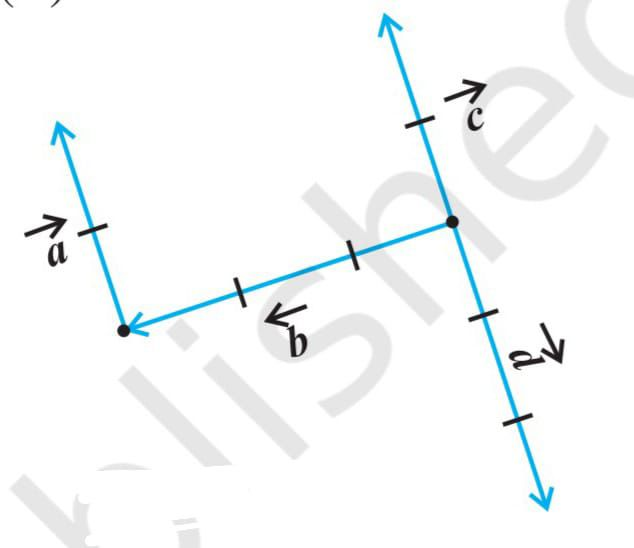
\includegraphics[width=\columnwidth]{figs/10.5.png}
\caption{10.5}                                          
\label{fig:10.5}                                       
\end{figure}
\item Find the values of $x,y$ and $z$ so that the vectors $\overrightarrow{a} = x\hat{i} +2\hat{j} +2\hat{k}$ and $\overrightarrow{b} = 2\hat{i} +y\hat{j} +\hat{k}$ are equal.
\item Let $\overrightarrow{a}=\hat{i} +2\hat{j}$ and $\overrightarrow{b} = 2\hat{i} +\hat{j}$. Is $\abs{\overrightarrow{a}} = \abs{\overrightarrow{b}}$? Are the vectors $\overrightarrow{a}$ and $\overrightarrow{b}$ equal?
\item Find unit vector in the direction of vector $\overrightarrow{a} = 2\hat{i} +3\hat{j} +\hat{K}$.
\item Find a vector in the direction of vector $\overrightarrow{a}=\hat{i} -2\hat{j}$ that has magnitude $7$ units.
\item Find the unit vector in the direction of the sum of the vectors, $\overrightarrow{a} = 2\hat{i} +2\hat{j} -5\hat{k}$ and $\overrightarrow{b} = 2\hat{i} +\hat{j} +3\hat{k}$.
\item Write the direction ratios of the vector $\overrightarrow{a} = \hat{i} +\hat{j} -\hat{k}$ and hence calculate its direction cosines.
\item Find the vector joining the points $P(2,3,0)$ and $Q(-1,-2,-4)$ directed from $P$ to $Q$.
\item Consider two points $P$ and $Q$ with position vectors $\overrightarrow{OP} = 3\overrightarrow{a}-2\overrightarrow{b}$ and $\overrightarrow{OQ}=\overrightarrow{a}+\overrightarrow{b}$. Find the position vector of a point $R$ which divides the line joining $P$ and $Q$ in the ratio $2:1$, 
\begin{enumerate}[label=(\roman*)]
\item internally, and 
\item externally.
\end{enumerate}
\item Show that the points $A(2\hat{i} -\hat{j} +\hat{k}), B(\hat{i} -3\hat{j}-5\hat{k}),C(3\hat{i} -4\hat{j} -4\hat{k})$ are the vertices of a right angled triangle.
\item Find the angle between two vectors $\overrightarrow{a}$ and $\overrightarrow{b}$ with magnitudes $1$ and $2$ respectively and when $\overrightarrow{a}\cdot \overrightarrow{b} = 1$.
\item Find angle $\theta$ between the vectors $\overrightarrow{a} = \hat{i} +\hat{j} -\hat{k}$ and $\overrightarrow{b} = \hat{i} -\hat{j}+\hat{k}$.
\item If $\overrightarrow{a} = 5\hat{i} -\hat{j} -3{k}$ and $\overrightarrow{b} = \hat{i} +3\hat{j} -5\hat{k}$, then show that the vectors $\overrightarrow{a}+\overrightarrow{b}$ and $\overrightarrow{a}-\overrightarrow{b}$ are perpendicular.
\item Find the projection of the vector $\overrightarrow{a} = 2\hat{i} +3\hat{j} +2\hat{k}$ on the vector $\overrightarrow{b} = \hat{i} +2\hat{j} +\hat{k}$.
\item Find $\abs{\overrightarrow{a}-\overrightarrow{b}}$, if two vectors $\overrightarrow{a}$ and $\overrightarrow{b}$ are such that $\abs{\overrightarrow{a}}=2, \abs{\overrightarrow{b}}=3$ and $\overrightarrow{a} \cdot \overrightarrow{b}=4$.
\item If $\overrightarrow{a}$ is a unit vector and $(\overrightarrow{x}-\overrightarrow{a}) \cdot (\overrightarrow{x}+\overrightarrow{a})=8$, then find $\abs{\overrightarrow{x}}$.
\item For any two vectors $\overrightarrow{a}$ and $\overrightarrow{b}$, we always have $\abs{\overrightarrow{a} \cdot \overrightarrow{b}} \leq  \abs{\overrightarrow{a}} \abs{\overrightarrow{b}}$ (Cauchy - Schwartz inequality).
\item For any two vectors $\overrightarrow{a}$ and $\overrightarrow{b}$, we always have $\abs{\overrightarrow{a}+\overrightarrow{b}} \leq \abs{\overrightarrow{a}} +\abs{\overrightarrow{b}}$ (triangle inequality).
\item Show that the points $A(-2\hat{i} +3\hat{j} +5\hat{k}), B(\hat{i}+2\hat{j} +3\hat{k}$ and $C(7{i} -\hat{k})$ are collinear.
\item Find $\abs{\overrightarrow{a} \times \overrightarrow{b}}$, if $\overrightarrow{a} = 2\hat{i} +\hat{j} +3\hat{k}$, and $\overrightarrow{b} = 3\hat{i} +5\hat{j} -2\hat{k}$.
\item Find a unit vector perpendicular to each of the vectors $(\overrightarrow{a} +\overrightarrow{b})$ and $(\overrightarrow{a} -\overrightarrow{b})$, where $\overrightarrow{a}=\hat{i} +\hat{j} +\hat{k}, \overrightarrow{b} = \hat{i} +2\hat{j} +3\hat{k}$.
\item Find the area of a triangle having the points $A(1,1,1), B(1,2,3)$ and $C(2,3,1)$ as its vertices.
\item Find the area of a parallelogram whose adjacent sides are given by the vectors $\overrightarrow{a}=3\hat{i} +\hat{j} +4\hat{k}$ and $\overrightarrow{b}=\hat{i} -\hat{j} +\hat{k}$.
\item Write all the unit vectors in $XY$-plane.
\item If $\hat{i}+\hat{j}+\hat{k}, 2\hat{i}+5\hat{j}, 3\hat{i}+2\hat{j}-3\hat{k}$ and $\hat{i}-6\hat{j}-\hat{k}$ are the position vectors of points $A, B, C$ and $D$ respectively, then find the angle between $\overrightarrow{AB}$ and $\overrightarrow{CD}$. Deduce that $\overrightarrow{AB}$ and $\overrightarrow{CD}$ are collinear.
\item Let $\overrightarrow{a}, \overrightarrow{b},$ and $ \overrightarrow{c}$ are three vectors such that $\abs{\overrightarrow{a}}=3, \abs{\overrightarrow{b}}=4 \abs{\overrightarrow{c}}=5$ and each one of them being perpndicular to the sum of the other to, find $\abs{\overrightarrow{a}+\overrightarrow{b}+\overrightarrow{c}}$.
\item Three vectors $\overrightarrow{a}, \overrightarrow{b}$ and $\overrightarrow{c}$ satisfy the condition $\overrightarrow{a} +\overrightarrow{b} +\overrightarrow{c} =0$. Evaluate the quantity $\mu = \overrightarrow{a}\cdot \overrightarrow{b} +\overrightarrow{b} \cdot \overrightarrow{c} +\overrightarrow{c} \cdot \overrightarrow{a}$, if $\abs{\overrightarrow{a}}=3, \abs{\overrightarrow{b}}=4$ and $\abs{\overrightarrow{c}}=2$. 
\item If with reference to the right handed system of mutually perpendicular unit vectors $\hat{i},\hat{j}$ and $\hat{k}, \overrightarrow{\alpha} = 3\hat{i} -\hat{j}, \overrightarrow{\beta}= 2\hat{i} +\hat{j} -3\hat{k}$, then express $\overrightarrow{\beta}$ in the form $\overrightarrow{\beta} = \overrightarrow{\beta_1} +\overrightarrow{\beta_2}$ where $\overrightarrow{\beta_1}$ is parallel to $\overrightarrow{\alpha}$ and $\overrightarrow{\beta_2}$ is perpendicular to $\overrightarrow{\alpha}$.
\end{enumerate}
\end{document}
